\documentclass[12pt,a4paper]{article}
\usepackage[utf8]{inputenc}
\usepackage[T1]{fontenc}
\usepackage{amsmath}
\usepackage{amsfonts}
\usepackage{amssymb}
\usepackage{ stmaryrd }
\usepackage{amsthm}
\usepackage{graphicx}
\usepackage{subfigure}
\usepackage{float}
\newtheorem*{lemma}{Lemma}
\newtheorem*{theorem}{Theorem}
\newtheorem*{corollary}{Corollary}
\newtheorem*{prf}{\textbf{Proof}}
\usepackage{caption}
\DeclareMathOperator{\n}{\nabla}
\DeclareMathOperator{\E}{\mathrm{E}}
\DeclareMathOperator{\xyz}{\textbf{numpy.random.normal()}}
\title{CS331-HW10-Lukang-Sun}
\begin{document}
	\maketitle
	\paragraph{p1.}
	(see Figure $\ref{img2}$.)
	a = [matrix([[0.1]]), matrix([[0.424466]]), matrix([[0.77981303]]), matrix([[0.20033184]]), matrix([[0.51116473]]), matrix([[0.2604399]]), matrix([[0.97100656]]), matrix([[0.21263449]]), matrix([[0.26417151]]), matrix([[0.15995097]])]
	
	b = [matrix([[0.4231786]]), matrix([[0.524466]]), matrix([[0.17981303]]), matrix([[0.50033184]]), matrix([[0.71116473]]), matrix([[0.0604399]]), matrix([[0.37100656]]), matrix([[0.91263449]]), matrix([[0.66417151]]), matrix([[0.65995097]])]
	,$f=\frac{1}{10}\sum_{i=1}^{10}f_i(x,y),f_i(x,y)=\sin(x+a[i])+\cos(y+b[i])$, for the SGD method, I use SGD-US and L-SVRG-US. Initial point is init = matrix([[-0.5],[-0.2]]).
	\newline 
	(1)L-SVRG-US will converge to the optimal point, while SGD-US will only converge to a neighborhood of the optimal point, in graph (a), we can see the results verifies  prediction.
	\newline
	(2)in L-SVRG-US, p is bigger the trajectories will be more smooth, while p is smaller, the trajectories will fluctuate, in graph (b), we can see the results verifies  prediction.
	\begin{figure}
		\centering
		\subfigure[ ]{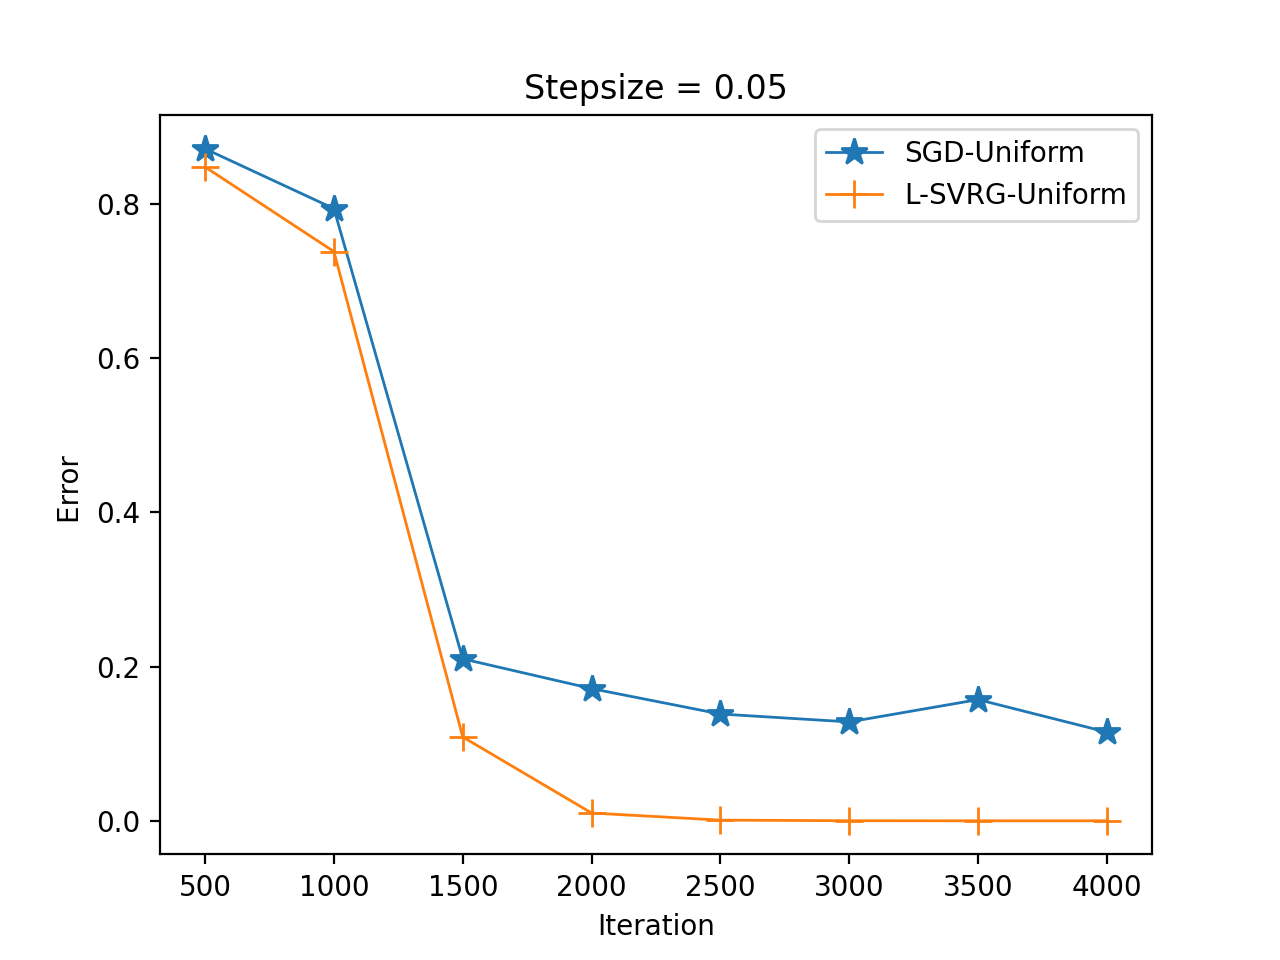
\includegraphics[width=6.7cm]{Figure_101.png}} 
		\subfigure[]{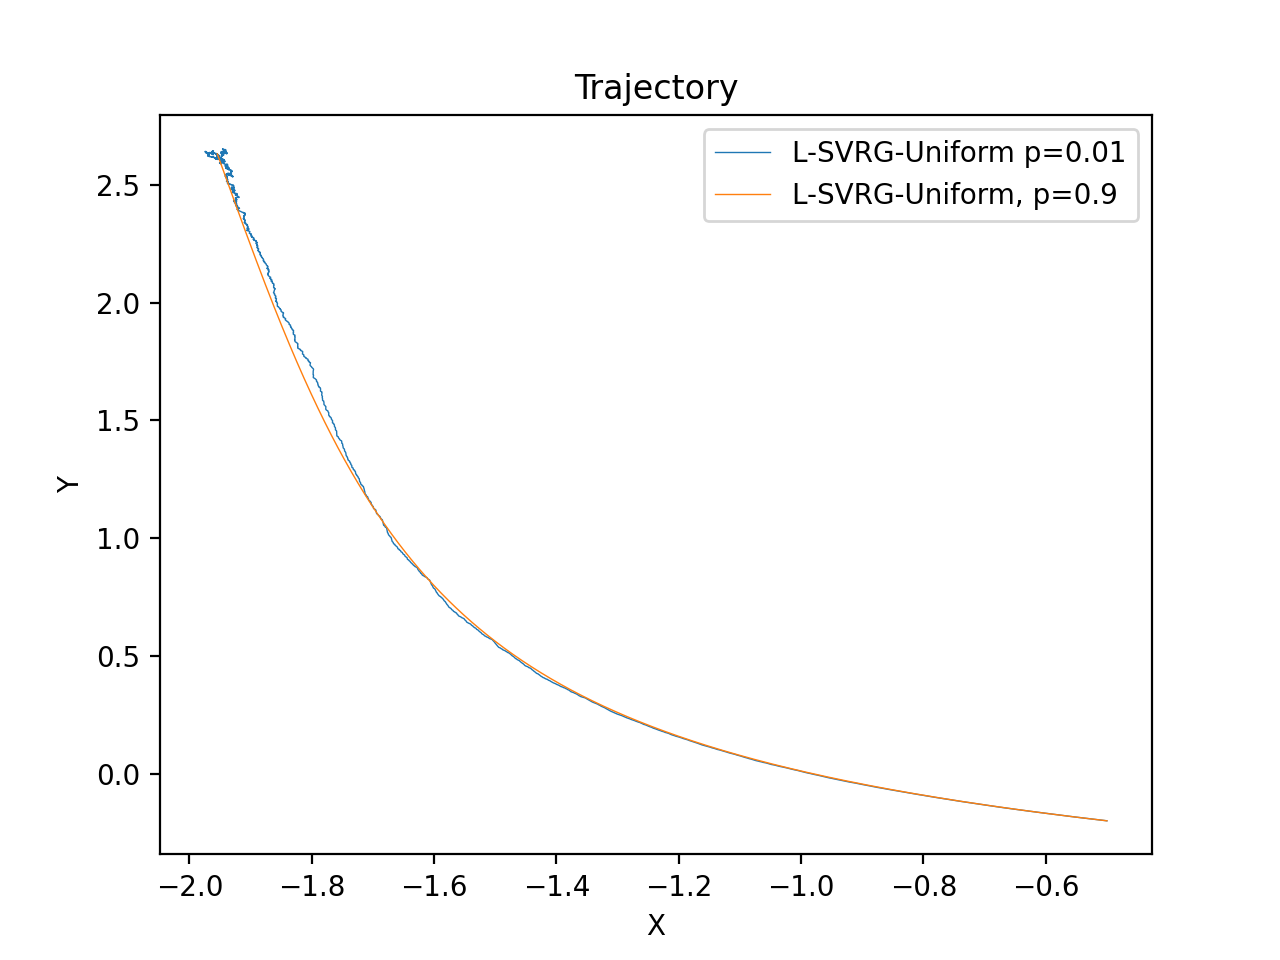
\includegraphics[width=6.7cm]{Figure_102.png}}
		
		
		\caption{ (a) shows $\E\left[||\nabla f||^2\right]$ changes in terms of iteration number K when set step size $\gamma = 0.05$,(b)  shows the trajectories of L-SVRG-US with different $p$.} %图片标题
		\label{img2}
	\end{figure}

	
	
	\paragraph{p2.}
	\begin{proof}
	The proof is almost the same as the proof of theorem 121.
	Since $f$ is $L$-smooth, we have
	$$
	\begin{aligned}
		f\left(x^{k+1}\right)-f^{\mathrm{inf}} & \leq f\left(x^{k}\right)-f^{\mathrm{inf}}+\left\langle\nabla f\left(x^{k}\right), x^{k+1}-x^{k}\right\rangle+\frac{L}{2}\left\|x^{k+1}-x^{k}\right\|^{2} \\
		& \stackrel{}{=} \quad f\left(x^{k}\right)-f^{\mathrm{inf}}-\gamma\left\langle\nabla f\left(x^{k}\right), g^{k}\right\rangle+\frac{L \gamma^{2}}{2}\left\|g^{k}\right\|^{2}
	\end{aligned}
	$$
	By applying expectation to both sides and subsequently using unbiasedness of $g^{k}$ and the assumed bound on the second moment of the stochastic gradient, we get
	$$
	\begin{aligned}
		&\mathrm{E}\left[f\left(x^{k+1}\right)-f^{\mathrm{inf}} \right]  \stackrel{}{\leq} \E\left [f\left(x^{k}\right)-f^{\mathrm{inf}}\right ]-\gamma\E\left[\left\|\nabla f\left(x^{k}\right)\right\|^{2}\right]+\frac{L \gamma^{2}}{2} \mathrm{E}\left[\left\|g^{k}\right\|^{2} \right] \\
		&\leq\E\left[ f\left(x^{k}\right)-f^{\mathrm{inf}}-\gamma\left\|\nabla f\left(x^{k}\right)\right\|^{2}+\frac{L \gamma^{2}}{2}\left[2 A\left(f\left(x^{k}\right)-f^{\mathrm{inf}}\right)+B_{1} \sigma^{k}+B_{2}\left\|\nabla f\left(x^{k}\right)\right\|^{2}+C\right] \right]\\
		&=\E\left[\left(1+L A \gamma^{2}\right)\left(f\left(x^{k}\right)-f^{\mathrm{inf}}\right)+\frac{L B_{1} \gamma^{2}}{2} \sigma^{k} -\left(\gamma-\frac{L B_{2} \gamma^{2}}{2}\right)\left\|\nabla f\left(x^{k}\right)\right\|_{2}^{2}+\frac{L C \gamma^{2}}{2}\right]
	\end{aligned}
	$$
	Choose any $M>0$ and define
	$$
	\Delta^{k+1} \stackrel{\text { def }}{=} f\left(x^{k+1}\right)-f^{\mathrm{inf}}+M \gamma^{2} \sigma^{k+1}
	$$
	
	$$
	\begin{aligned}
		&\mathrm{E}\left[\Delta^{k+1} \right] {\leq} \E\left[\left(1+L A \gamma^{2}+2 M \tilde{A} \gamma^{2}\right)\left(f\left(x^{k}\right)-f^{i n f}\right)+\left(\frac{L B_{1}}{2}+M \tilde{B}_{1}\right) \gamma^{2} \sigma^{k}\right]\\
		&-\E\left[\left(\gamma-\frac{L B_{2} \gamma^{2}}{2}-M \tilde{B}_{2} \gamma^{2}\right)\left\|\nabla f\left(x^{k}\right)\right\|^{2}+\frac{L C \gamma^{2}}{2}+M \tilde{C} \gamma^{2}\right]\\
		&=\E\left[a\left[f\left(x^{k}\right)-f^{\inf }+\frac{\frac{L B_{1}}{2}+M \tilde{B}_{1}}{a} \gamma^{2} \sigma^{k}\right]-b\left\|\nabla f\left(x^{k}\right)\right\|^{2}+c\right]
	\end{aligned}
	$$
	where
	$$
	\begin{aligned}
		&a \stackrel{\text { def }}{=} 1+L A \gamma^{2}+2 M \tilde{A} \gamma^{2} \\
		&b \quad \stackrel{\text { def }}{=} \quad \gamma-\frac{L B_{2} \gamma^{2}}{2}-M \tilde{B}_{2} \gamma^{2} \\
		&c \quad \stackrel{\text { def }}{=} \frac{L C \gamma^{2}}{2}+M \tilde{C} \gamma^{2}
	\end{aligned}
	$$
	In order to turn (1) into a recursion which has $\Delta^{k}$ on the right hand side, we need to make sure that
	$$
	\frac{\frac{L B_{1}}{2}+M \tilde{B}_{1}}{a} \leq M
	$$
	Fortunately, it is easy to see (prove this!) that we can make sure this holds by an appropriate choice of $M$. In particular, the last inequality  holds if we choose
	$$
	M \stackrel{\text { def }}{=} \frac{L B_{1}}{2\left(1-\tilde{B}_{1}\right)}=\frac{L \theta}{2}
	$$
	With this choice of $M$, we can continue from $(314)$ and obtain the recursion
	\begin{equation}
	\mathrm{E}\left[\Delta^{k+1} \right] \quad {\leq}\E\left[ a \Delta^{k}-b\left\|\nabla f\left(x^{k}\right)\right\|^{2}\right]+c
	\end{equation}
	By applying expectation to both sides of this, and using the tower property of expectation, we get the recursion
	\begin{equation}
	\begin{aligned}
		\mathrm{E}\left[\Delta^{k+1}\right] &=\mathrm{E}\left[\mathrm{E}\left[\Delta^{k+1} \mid x^{k}, \xi^{k}\right]\right] \\
		& {\leq} \quad a \mathrm{E}\left[\Delta^{k}\right]-b \mathrm{E}\left[\left\|\nabla f\left(x^{k}\right)\right\|^{2}\right]+c
	\end{aligned}
   \end{equation}
	We now apply Lemma 120 to recursion (2) with $X_{k}=\mathrm{E}\left[\Delta^{k}\right]$ and $Y_{k}=b \mathrm{E}\left[\left\|\nabla f\left(x^{k}\right)\right\|^{2}\right] .$ If we set $x=x^{k}$ with probability $p_{k}$ (where $p_{k}$ is as in Lemma 120), which means that $Y=Y_{k}$ with probability $p_{k}$, we conclude that
	\begin{equation}
	\begin{aligned}
		b \mathrm{E}\left[\|\nabla f(x)\|^{2}\right] &=\mathrm{E}[Y] \\
		&\leq \frac{a^{K}}{S_{K}} \Delta^{0}+c \\
		& \leq \frac{a^{K}}{K} \Delta^{0}+c
	\end{aligned}
   \end{equation}
	where the last inequality follows since $a \geq 1$, which implies that $S_{K} \geq K .$ We now evaluate the expressions for $b$ and $c$ in (3). First,
	\begin{equation}
	\begin{aligned}
		b \quad & {=} \gamma-\frac{L B_{2} \gamma^{2}}{2}-M \tilde{B}_{2} \gamma^{2} \\
		& {=} \gamma-\frac{\gamma}{2}\left(L B_{2} \gamma+L \theta \tilde{B}_{2} \gamma\right) \\
		& \geq \frac{\gamma}{2}
	\end{aligned}
	\end{equation}
	where the last inequality holds by setting
	$$
	\gamma \leq \frac{1}{L\left(B_{2}+\theta \tilde{B}_{2}\right)}
	$$
	Moreover,
	\begin{equation}
	c {=} \frac{L C}{2} \gamma^{2}+M \tilde{C} \gamma^{2} {=} \frac{L}{2}(C+\theta \tilde{C}) \gamma^{2}
\end{equation}
	By plugging the bound (4) on $b$ and expression (5) for $c$ into (3), we obtain the result.
	
	\end{proof}
	
	\paragraph{p3.}
	\begin{proof}
	By lecture, we have 
	$$
	E\left[\|\nabla f(x)\|^{2}\right] \leq \frac{2\left(f\left(x^{0}\right)-f^{\mathrm{inf}}\right)}{K} \times \max \{\underbrace{\sqrt{\frac{4}{3} \frac{1-p}{p} \alpha(c+1)}}_{M_{1}} ,L \underbrace{\left(B_{2}+\frac{B_{1} \tilde{B}_{2}}{1-\tilde{B}_{1}}\right)}_{M_{2}}\}
	$$
	$$
	M_2\leq L\left(1+\frac{3}{c+1}+\frac{4(1-p)}{p c}\right)
	$$
	$$
	\alpha \stackrel{\operatorname{def}}{=} \frac{(n-\tau) L_{\mathrm{avg}}^{2}}{(n-1) \tau},
	$$
	if we let $p=0.5, c=1$, then $M_1 = \sqrt{\frac{8}{3}}n^{-1/3}L_{avg}, M_2\leq 6.5L$, so $\max\left\{M_1,M_2\right\}\leq 6.5L$, when $n$ is large. So we need $\mathcal{O}\left(\frac{1}{\epsilon^2}\right)$ steps to make the error less than $\epsilon^2$, each step's computation is $n^{2/3}$, so, the total complexity is $\mathcal{O}\left(n^{2 / 3} / \varepsilon^{2}\right)$.
	\end{proof}	

	\paragraph{p4.}
	\begin{theorem}
		Let Assumption 8 (L-smoothness and $f \geq f^{\text {inf }}$ ), PL-condition ($||\nabla f(x)||^2_2\geq 2\mu(f(x)-f(x^{\star}))$) and Assumption $11\left(\sigma^{k}\right.$ assumption for nonconvex functions) be satisfied. Choose constant stepsize $\gamma$ satisfying
		\begin{equation*}
			0<\gamma \leq \min\left\{\frac{1}{\frac{L B_{2}}{2}+M \tilde{B}_{2}},\frac{\mu}{L A+2 M A+\mu L B_{2}+2 \mu M \tilde{B}_{2}}\right\}
		\end{equation*}
Then
\begin{equation*}
	\E\left[\Delta^k\right]\leq (1-\mu\gamma)^k\Delta^0+\frac{c}{\mu\gamma}
\end{equation*}
	where $c \stackrel{\text { def }}{=} \frac{L C \gamma^{2}}{2}+M \tilde{C} \gamma^{2},M=\frac{L B_{1}}{2\left(a-2 \mu b-\tilde{B}_{1}\right)},a  \stackrel{\text { def }}{=} 1+L A \gamma^{2}+2 M \tilde{A} \gamma^{2},b  \stackrel{\text { def }}{=} \quad \gamma-\frac{L B_{2} \gamma^{2}}{2}-M \tilde{B}_{2} \gamma^{2},\Delta^{k} \stackrel{\text { def }}{=} f\left(x^{k}\right)-f^{\inf }+M \gamma^{2} \sigma^{k}$,
	\end{theorem}
	\begin{proof}
		Since $f$ is $L$-smooth, we have
		\begin{equation}
		\begin{aligned}
			f\left(x^{k+1}\right)-f^{\text {inf }} & \leq f\left(x^{k}\right)-f^{\text {inf }}+\left\langle\nabla f\left(x^{k}\right), x^{k+1}-x^{k}\right\rangle+\frac{L}{2}\left\|x^{k+1}-x^{k}\right\|^{2} \\
			& \stackrel{(295)}{=} f\left(x^{k}\right)-f^{\text {inf }}-\gamma\left(\nabla f\left(x^{k}\right), g^{k}\right\rangle+\frac{L \gamma^{2}}{2}\left\|g^{k}\right\|^{2} .
		\end{aligned}
		\end{equation}
		By applying expectation to both sides of $(6)$ and subsequently using unbiasedness of $g^{k}$ and the assumed bound $(297)$ (from lecture)on the second moment of the stochastic gradient, we get
		\begin{equation}
		\begin{aligned}
			\mathrm{E}\left[f\left(x^{k+1}\right)-f^{\mathrm{inf}} \mid x^{k}, \xi^{k}\right] & \stackrel{(6)}{\leq} f\left(x^{k}\right)-f^{\mathrm{inf}}-\gamma\left\|\nabla f\left(x^{k}\right)\right\|^{2}+\frac{L \gamma^{2}}{2} \mathrm{E}\left[\left\|g^{k}\right\|^{2} \mid x^{k}, \xi^{k}\right] \\
			& \stackrel{(297)}{\leq} f\left(x^{k}\right)-f^{\mathrm{inf}}-\gamma\left\|\nabla f\left(x^{k}\right)\right\|^{2} \\
			&+\frac{L \gamma^{2}}{2}\left[2 A\left(f\left(x^{k}\right)-f^{\mathrm{inf}}\right)+B_{1} \sigma^{k}+B_{2}\left\|\nabla f\left(x^{k}\right)\right\|^{2}+C\right] \\
			=&\left(1+L A \gamma^{2}\right)\left(f\left(x^{k}\right)-f^{\mathrm{inf}}\right)+\frac{L B_{1} \gamma^{2}}{2} \sigma^{k} \\
			&-\left(\gamma-\frac{L B_{2} \gamma^{2}}{2}\right)\left\|\nabla f\left(x^{k}\right)\right\|^{2}+\frac{L C \gamma^{2}}{2}
		\end{aligned}
		\end{equation}
	Choose any $M>0$ and define
	\begin{equation}
	\Delta^{k+1} \stackrel{\text { def }}{=} f\left(x^{k+1}\right)-f^{\text {inf }}+M \gamma^{2} \sigma^{k+1}
	\end{equation}
	by combining inequality (7) with assumption (298), we get 
	\begin{equation}
	\begin{aligned} E\left[\Delta^{k+1} \mid x^{k}, \xi^{k}\right]& \quad \stackrel{(306)+(298)}{\leq} \underbrace{\left(1+L A \gamma^{2}+2 M \tilde{A} \gamma^{2}\right)}_{=a}\left(f\left(x^{k}\right)-f^{\mathrm{inf}}\right) +\left(\frac{L B_{1}}{2}+M \tilde{B}_{1}\right) \gamma^{2} \sigma^{k} \\ 
		&-\underbrace{\left(\gamma-\frac{L B_{2} \gamma^{2}}{2}-M \tilde{B}_{2} \gamma^{2}\right)}_{=b}\left\|\nabla f\left(x^{k}\right)\right\|^{2}+\underbrace{\frac{L C \gamma^{2}}{2}+M \tilde{C} \gamma^{2}}_{=c}\\
	&  \quad \stackrel{\text{PL-condition}}{\leq}  (a-2\mu b)\left[f\left(x^{k}\right)-f^{\mathrm{inf}}+\frac{\frac{L B_{1}}{2}+M \tilde{B}_{1}}{a-2\mu b} \gamma^{2} \sigma^{k}\right]+c	
 \end{aligned}
	\end{equation}
	where 
	$$
	\begin{array}{ll}
		a & \stackrel{\text { def }}{=} 1+L A \gamma^{2}+2 M \tilde{A} \gamma^{2} \\
		b & \stackrel{\text { def }}{=} \quad \gamma-\frac{L B_{2} \gamma^{2}}{2}-M \tilde{B}_{2} \gamma^{2} \\
		c & \stackrel{\text { def }}{=} \frac{L C \gamma^{2}}{2}+M \tilde{C} \gamma^{2},
	\end{array}
	$$
	we also require $b\geq 0$, that is $\gamma\leq \frac{1}{\frac{LB_2}{2}+M\tilde{B}_2}$.
	In order to turn (314) into a recursion which has $\Delta^{k}$ on the right hand side, we need to make sure that
	$$
	\frac{\frac{L B_{1}}{2}+M \tilde{B}_{1}}{a-2\mu b} \leq M
	$$
	We can choose $M=\frac{LB_1}{2(a-2\mu b-\tilde{B}_1)}$.
	With this choice of $M$, we can continue from $(10)$ and obtain the recursion
	\begin{equation}
	\mathrm{E}\left[\Delta^{k+1} \mid x^{k}, \xi^{k}\right] \leq  (a-2\mu b) \Delta^{k}+c
	\end{equation}
	By applying expectation to both sides of this, and using the tower property of expectation, we get the recursion
	$$
	\begin{aligned}
		\mathrm{E}\left[\Delta^{k+1}\right] &=\mathrm{E}\left[\mathrm{E}\left[\Delta^{k+1} \mid x^{k}, \xi^{k}\right]\right] \\
		&(\leq (a-2\mu b) \mathrm{E}\left[\Delta^{k}\right]+c
	\end{aligned}
	$$
	Finally,
	\begin{equation}
		\E\left[\Delta^{k}\right]\leq (a-2\mu b)^k\Delta^0+c\sum_{i=0}^{k}(a-2\mu b)^i
	\end{equation}
	by choosing $\gamma\leq \frac{\mu}{LA+2MA+\mu L B_2+2\mu M\tilde{B}_2}$, we will have $a-2\mu b\leq 1-\mu\gamma$
	so from $(11)$, we have 
	\begin{equation}
		\E\left[\Delta^k\right]\leq (1-\mu\gamma)^k\Delta^0+\frac{c}{\gamma \mu}
	\end{equation}
	\end{proof}
	
\end{document}